
\chapter{ASSIGNMENTS}
\section*{\centering\LARGE{LAB ASSIGNMENT 01}}

\subsection*{\underline{Aim}}
Refer Chapter 7 of first reference to develop the problem under consideration and justify feasibility using concepts of knowledge canvas and IDEA Matrix. 
\subsection*{\underline{Project}}
Voice Controlled Personal Assistant Device and Connecting IOT Devices \\

\begin{table}[ht]
\caption{Project Canvas}
\begin{tabular}{ |p{5cm}|p{5cm}|p{5cm}|  }
 \hline
 \textbf{Purpose} & \textbf{Goals} & \textbf{Users}\\
 \hline
To reduce the human efforts & To produce precise desired output with given minimal input and greater time-efficiency & All Age-Group Humans\\

To Connect IOT Devices in the vicinity & To interface the device with the IOT devices for home automation & Industries and Enterprises \\
 
 \hline
 \end{tabular}
 \end{table}
 
 \begin{table}

\vspace{0.5cm} 
 
\begin{tabular}{ |p{5cm}|p{5cm}|p{5cm}|  }
 \hline
 \textbf{Actions} & \textbf{Deliverables} & \textbf{Risks} \\
 \hline
 To define functionality of device along with respective vocal commands  & SRS \& Project Design & Features should work in harmony and both time and space efficiency\\


  Work on different Modules of Project to build an integrated system & Project Report \& Project & Device may not be able to perform the service according to command\\
   \hline
 
 \end{tabular}
 \end{table}
\vspace{0.5cm} 
\begin{table}
 \begin{tabular}{ |p{5cm}|p{5cm}|p{5cm}|  }
 \hline
 \textbf{Milestones} & \textbf{Constraints} & \textbf{Scope} \\
 \hline
 Synopsis, Abstract, Report & All Functionality well defined with all possible voice commands which & Commands limited to only English\\

  Coding and Final Software  & Device should work in any environment & Limited to quality of the vocal commands\\ 
   \hline
 \end{tabular}
\end{table} 
\pagebreak
\newpage
\noindent\\\\
\\\\
\\\\
\\\\
\\\\
\\\\
\\\\
\\\\
\\\\
\\\\
\\\\
\section*{\centering\LARGE{LAB ASSIGNMENT 02}}
\subsection*{\underline{Aim}}
Project problem statement feasibility assessment using NP-Hard, NP-Complete or satisfy ability issues using modern algebra and/or relevant mathematical models.

\subsection*{\underline{Feasibility Theory}}
The feasibility of the project can be defined as the measure of our project whether it is viable or not.It includes various different types of feasibility as follows:
\begin{itemize}
\item \textbf{Performance:}\\
In this we check whether the proposed system is capable of performing all the functional requirements as mentioned in system features in SRS.If our system is performing the functional requirements appropriately then it's performance is feasible.Here we also check the accuracy and efficiency of the system based on various STT-TTS Engines.
\item \textbf{Technical:}\\
In this we check whether the technical specification provided that is hardware and software requirements are minimum requirements for our platform to run successfully without any error regarding the system configuration. Also the voice commands are suffice to call a predefined functionality module and features are performed effectively.
\item \textbf{Economical:}\\
In this we check the cost per line of code, also the cost for storage of hardware required and cost related to the run time of the system.Apart from this since no large database transactions are needed apart from minimum system data which will be required for profilication.

\end{itemize}
\noindent
\subsection*{\underline{Feasibility on basis of Class of Problem}}
\hspace{3em}Complexity classes are one way to talk about how difficult or easy a problem is.
Complexity theory gets very technical but the basics are actually extraordinarily
intuitive, and it's possible to understand the P versus NP issue with very little
math background.\\

\noindent
If there is a fast solution to the search version of a problem then the problem is
said to be Polynomial time, or P for short. If there is a fast solution to the verification version of a problem then the problem is said to be Non deterministic Polynomial time,
or NP for short. The question of "P=NP" is then the question of whether these sets are identical.\\

\noindent
Some problems can be translated into one another in such a way that a fast
solution to one problem would automatically give us a fast solution to the
other. There are some problems that every single problem in NP can be
translated into, and a fast solution to such a problem would automatically give
us a fast solution to every problem in NP. This group of problems are known as
NP Hard.Some problems in NP Hard
are actually not themselves in NP; the
group of problems that are in both NP and NP Hard
is called NP Complete

\subsection*{\underline{Classes of problems}}
\begin{itemize}
\item \textbf{NP}\\
A lot of programs that don't (necessarily) run in polynomial time
on a regular computer, but do run in polynomial time on a non deterministic
Turing machine. These programs solve problems in NP, which stands for
non deterministic polynomial time.An equivalent way to define NP is by pointing to the problems that can be
verified in polynomial time.

\item \textbf{NP Hard}\\
If a problem is NP hard,
this means I can reduce any problem in NP to that problem. This means if I can solve that problem, I can easily solve any problem in NP. If we could solve an NP hard
problem in polynomial time, this would
prove P = NP.

\item \textbf{NP Complete}\\
A problem is NP complete
if the problem is both
NP hard, and in NP.
\end{itemize}

\noindent
\hspace{3em}Our system satisfies not only problems of bringing different services under one platform as well as we are adding many functionality which are not provided by other personal assistant devices and connecting IOT devices as well as extending usability by providing and Android application as well.\\

\noindent
\hspace{3em}Since we have a fast solution to convert the speech into a recognizable functionality it is said to be P type problem capable to solve a part in polynomial time also the servicing the functionality doesn't has a fast solution so it  is not a NP complete problem.
\subsection*{\underline{Relation Between Classes of Problems}}
 \begin{figure}[H]
    \centering
  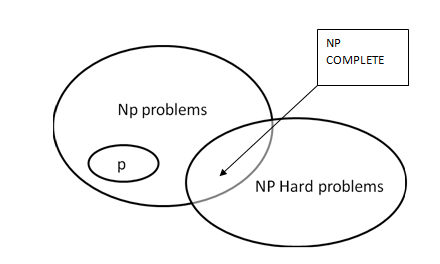
\includegraphics[scale=0.9]{nprelation.PNG}\\
  \caption{Relation between Classes of Problems}

\end{figure}
     \subsection*{\underline{Mathematical Model}}
  \textbf{Mathematical Formulation:}\\
Let the M i the universal states which contains, \\
    \textbf{M = \{Q, S, F, Q1 , Qf \}} \newline
    where, \\
    \newline
    		Q = No. of states \{Q1,Q2,Q3,Q4,Q5,Q6,Q7,Q8\}\\
    		X = No. of states \{X1, X2, X3, X4\}\\
    		Q1 = Initial State.\\
    		S = Success state.\\
    		F = Failure state.\\
    		\newline
    where,\\ 
    \newline
    Q1= Start.\\
     \newline
    Q2 = Initialize assistant by calling action word. \\
    \newline
    Q3 = Once initialized, give input in the speech format.\\
    \newline
    Q4 = Processing of speech into text.\\
    \newline 
    Q5 = Text is compared with commands.\\
    \newline
    Q6 = Perform action according to command.\\
    \newline 
    Q7 = Convert the action into speech.\\
    \newline 
    Q8 = Give output in the speech format.\\
    \newline
    X1 = Connect Personal AI Device to mobile application.\\
    \newline
    X2 = Update To-Do list, Calender, Alarm, reminder, etc.\\
    \newline
    X3 = Updated data is sent to cloud server.\\
    \newline
    X4 = According to the data sent, AI Device will take action.\\
    \newline

\noindent   
\textbf{Failure Conditions:}  F = \{F1,F2,F3\} \newline
\begin{itemize}
\item F1  = Failure if the device is not initialised due to noisy background.
\item F2 = Connection with android app failed.
\item F3 = Server down failure or cannot retrieve data from server.
\end{itemize}

\noindent
 \textbf{Success Conditions:} S = \{S1\}
    \begin{itemize}
    		\item S1 = Success after the data is assimilated and output is produced accordingly.
	\end{itemize}     

\subsection*{\underline{Activity Diagram}}
\begin{tikzpicture}[node distance = 6cm, auto, line width=1pt,>=latex]
    % Place nodes
    \node [cloud] (Q1) {Q1};
    \node [cloud, right of=Q1] (Q2) {Q2};
    \node [cloud, right of=Q2] (Q3) {Q3};
    \node [cloud, right of=Q3] (f1) {F1};
    \node [cloud, below of=f1] (Q4) {Q4};
    \node [cloud, below of=Q4] (Q5) {Q5};
    \node [cloud, below of=Q5] (Q6) {Q6};
    \node [cloud, below of=Q6] (Q7) {Q7};
    \node [cloud, below of=Q7] (Q8) {Q8};
    \node [cloud, left of=Q4] (x1) {X1};
    \node [cloud, left of=x1] (f2) {F2};
    \node [cloud, left of=Q5] (x2) {X2};
    \node [cloud, left of=Q6] (x3) {X3};
    \node [cloud, left of=x3] (f3) {F3};
    \node [cloud, left of=Q7] (x4) {X4};
    \node [cloud, below of=Q7] (Q8) {};
    % Draw edges
    \path [line] (Q1) -- (Q2);
    \path [line] (Q2) -- (Q3);
    \path [line] (Q3) -- (Q4);
    \path [line] (Q3) -- (f1);
    \path [line] (Q4) -- (Q5);
    \path [line] (x1) -- (f2);
    \path [line] (x3) -- (f3);
    \path [line] (Q5) -- (Q6);
    \path [line] (Q6) -- (Q7);
    \path [line] (Q7) -- (Q8);
    \path [line] (x1) -- (x2);
    \path [line] (x2) -- (x3);
    \path [line] (x3) -- (x4);
    \path [line] (x1) -- (Q5);
    \path [line] (x4) -- (Q7);
    \path [line] (f2) -- (Q1);
    \path [line] (f3) -- (x1);

    \end{tikzpicture}


\newpage
\section*{\centering\LARGE{Lab Assignment 03}}
\subsection*{\underline{Aim}}
\noindent
Use of divide and conquer strategies to exploit distributed/parallel/concurrent processing of the above to identify objects, morphisms, overloading in functions (if any), and functional relations and any other dependencies (as per requirements).
\subsection*{\underline{Concept}}
\hspace*{3em}A divide and conquer algorithm works by recursively breaking down a problem into two or more sub-problems of the same (or related) type (divide), until these become simple enough to be solved directly (conquer). So have divided our problem based on modules used and those are:
\begin{itemize}
\item IOT box
\item Android Smart-phone application
\item Voice input and processing.
\item Get data from Firebase cloud DB.
\item Generating speech using TTS task model.
\end{itemize}

\noindent
Divide and conquer (D\&C) is an algorithm design paradigm based on multi-branched recursion. So we have to recursively divide our problem into  sub-problems  of the same (or related) type (divide), until these sub-problem become simple enough to be solved directly (conquer). The solutions to the sub-problems are then combined to give a solution to the original problem.\\

\noindent
In our project we have divided our project into 4 phases which are : Data collection in the form of voice, voice analysis and conversion to text, data storage and processing, and generating speech from the processed text output. Now, in  Data collection in the form of voice, the data is stored as input for next step. \\

\noindent
In IoT box, tasks are divided in three modules and data transmission takes place through nRF24L01 transceiver. Task modules used in IoT box are 
\begin{itemize}
\item Servo Motor for mechanical movement for object, in our case: Curtains.
\item Switching on and off Neo-pixel ring.
\item LED display : Displays the data.
\end{itemize}

\noindent
Android application helps the user to share his personalized data through android application with ease from anywhere. The data transfer and processing is done through network adapter inbuilt APIs. This data generated is stored in firebase cloud storage and is available for the main system to access. All these tasks are being done in parallel to each other.\\

\noindent
All the data stored in Firebase cloud server is accessible to main system and can be retrieved and process as per required. The need of given data is also processed in parallel to continuous fetching of data from the server.\\

\noindent
The input voice is continuously processed and converted to text using STT along with the identifying and processing the commands using Python Script in background. The output then generated is converted from simple text to speech using TTS.\\
     
    \begin{figure}[H]
    \includegraphics[scale=0.60]{sysflow.png}\\
    \caption{Data-flow Diagram}
    \end{figure}

\newpage
\section*{\centering\LARGE{Lab Assignment 04}}
\subsection*{\underline{Aim}}
Use of above to draw functional dependency graphs and relevant Software modelling methods, techniques including UML diagrams or other necessities using appropriate tools.
    \subsection*{USE CASE DIAGRAM}
    \begin{figure}[H]
    \centering
  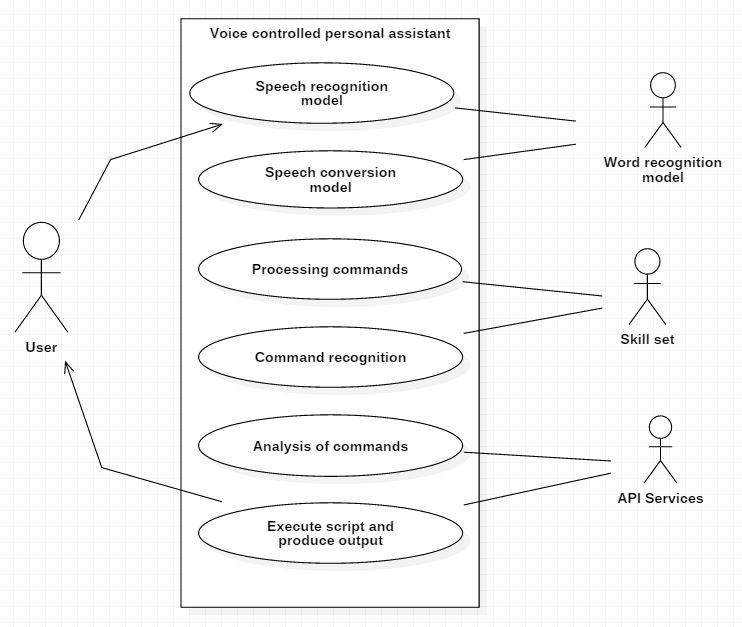
\includegraphics[scale=0.75]{UseCase.JPG}\\
  \caption{Use Case Diagram}
  \end{figure}
    \pagebreak
    
        \subsection*{CLASS DIAGRAM}
    \begin{figure}[H]
    \centering
  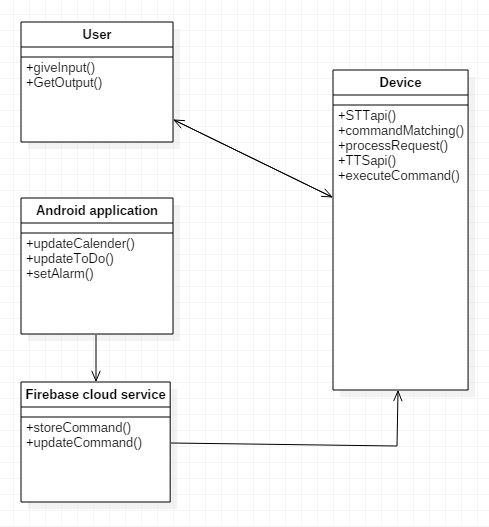
\includegraphics[scale=0.75]{Class.JPG}\\
  \caption{Class Diagram}
\end{figure}

    \subsection*{ACTIVITY DIAGRAM}
    \begin{figure}[H]
  \centering
  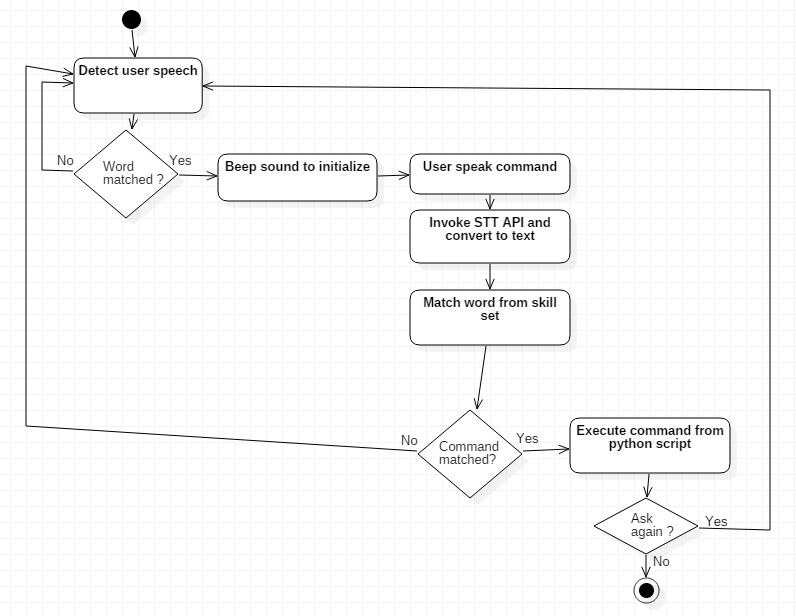
\includegraphics[scale=0.75]{Activity.JPG}\\
  \caption{Activity Diagram}
\end{figure}
   \pagebreak 
   
    \subsection*{DEPLOYMENT DIAGRAM}
     \begin{figure}[H]
  \centering
  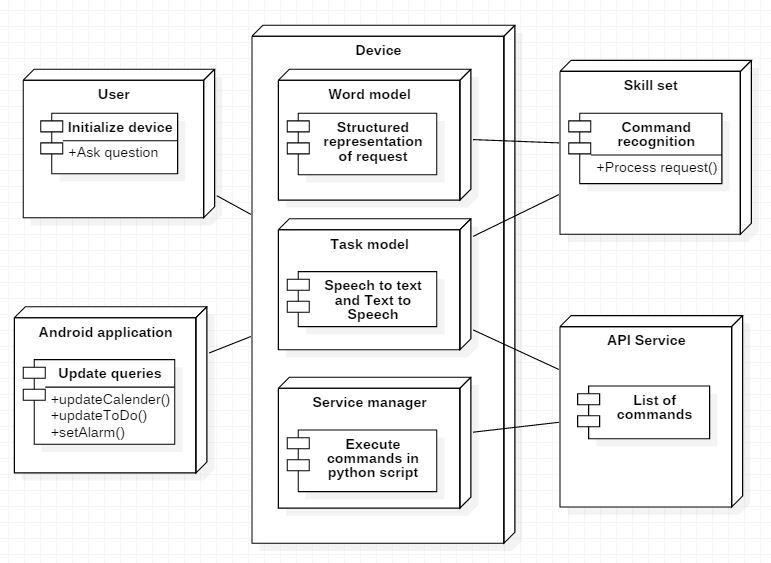
\includegraphics[scale=0.75]{Deployment.JPG}\\
  \caption{Deployment Diagram}
  \end{figure}
  \pagebreak
    
    \subsection*{SEQUENCE DIAGRAM}
    \begin{figure}[H]
  \centering
  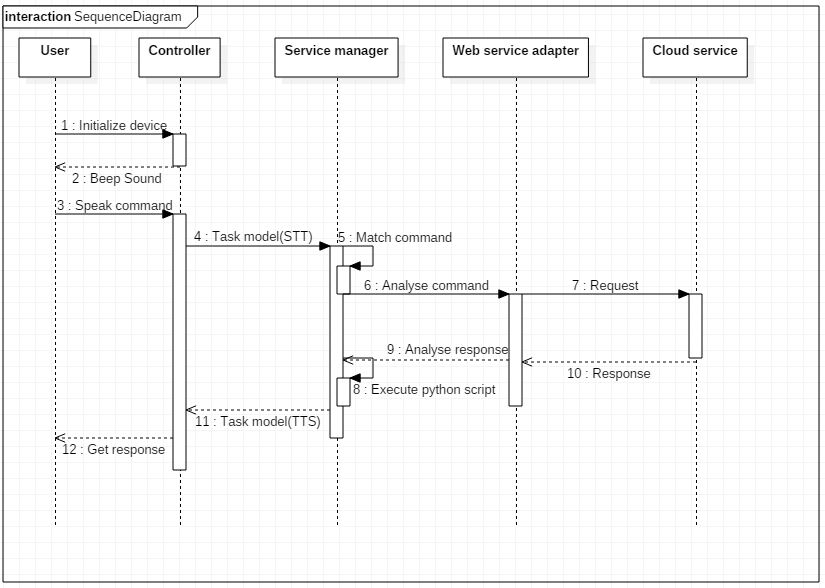
\includegraphics[scale=0.65]{Sequence.JPG}\\
  \caption{Sequence Diagram}
\end{figure}
 \pagebreak   
 
    \subsection*{STATE CHART DIAGRAM}
    \begin{figure}[H]
  \centering
  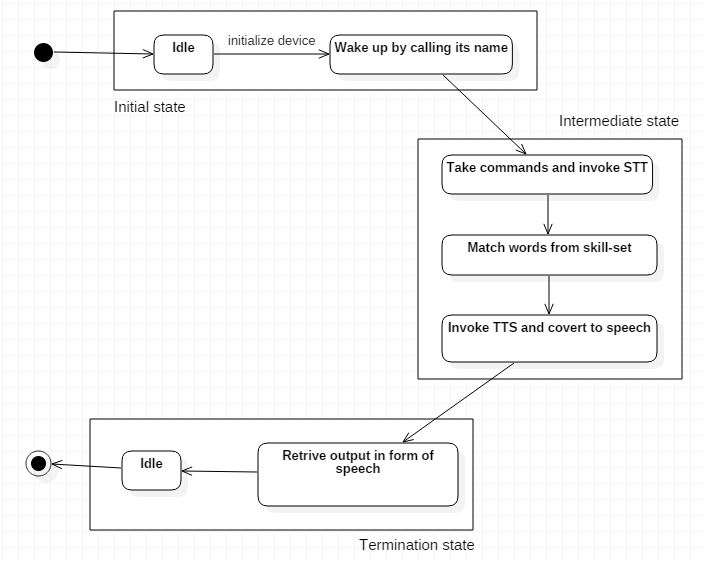
\includegraphics[scale=0.7]{StateChart.JPG}\\
  \caption{State Chart Diagram}
\end{figure}
\pagebreak

\newpage
\section*{\centering\LARGE{Lab Assignment 05}}
\subsection*{\underline{Aim}}
Testing of project problem statement using generated test data (using mathematical models, GUI, Function testing principles, if any) selection and appropriate use of testing tools, testing of UML diagram's reliability.
\noindent
\subsection*{\underline{Testing}}
\textbf{WHAT IS SOFTWARE TESTING?}\\
\hspace{5em} Software testing is a process of verifying and validating that a software application or program\\
1. Meets the business and technical requirements that guided its design and development, and\\
2. Works as expected.\\\\
Software testing also identifies important defects, flaws, or errors in the application code that must be fixed.\\
\newline
\noindent
\hspace{5em}Software testing has three main purposes: verification, validation, and defect finding.
\begin{itemize}
 \item The verification process confirms that the software meets its technical specifications. A “specification” is a
description of a function in terms of a measurable output value given a specific input value under specific
preconditions. A simple specification may be along the line of “a SQL query retrieving data for a single
account against the multi-month account-summary table must return these eight fields $<$list$>$ ordered by
month within 3 seconds of submission.”
 \item The validation process confirms that the software meets the business requirements. A simple example of a
business requirement is “After choosing a branch office name, information about the branch’s customer account managers will appear in a new window. The window will present manager identification and summary information about each manager’s customer base: $<$list of data elements$>$.” Other requirements
provide details on how the data will be summarized, formatted and displayed.
 \item A defect is a variance between the expected and actual result. The defect’s ultimate source may be traced
to a fault introduced in the specification, design, or development (coding) phases. 
\end{itemize}
\newpage

\noindent
\textbf{Software testing answers questions that development testing and code reviews can’t}
\begin{enumerate}
\item Does it really work as expected?
\item Does it meet the users’ requirements?
\item Is it what the users expect?
\item Do the users like it?
\item Is it compatible with our other systems?
\item How does it perform?
\item How does it scale when more users are added?
\item Which areas need more work?
\item Is it ready for release?
\end{enumerate}
\textbf{What can we do with the answers to these questions?}
\begin{enumerate}
\item Save time and money by identifying defects early
\item Avoid or reduce development downtime
\item Provide better customer service by building a better application
\item Know that we’ve satisfied our users’ requirements
\item Build a list of desired modifications and enhancements for later versions
\item Identify and catalog reusable modules and components
\item Identify areas where programmers and developers need training 
\end{enumerate}

\subsection*{\underline{The Test Plan}}
\noindent
\hspace{3em}
The test plan is a mandatory document. You can’t test without one. For simple, straight-forward projects the plan
doesn’t have to be elaborate but it must address certain items. As identified by the “American National Standards
Institute and Institute for Electrical and Electronic Engineers Standard 829/1983 for Software Test Documentation”,
the following components should be covered in a software test plan.\\
    
\begin{table}[ht]
    \caption{Test Plan}
    \begin{tabular}{ |p{5cm}|p{5cm}|p{5cm}|  }
    \hline
    \textbf{Component} & \textbf{Description} & \textbf{Purpose}\\
    \hline
    Responsibilities & Specific people who are and their assignments & Assigns responsibilities and keeps everyone on track and focused\\\hline

    Assumptions & Code and systems status and availability & Avoids misunderstandings about schedules \\\hline
    
    Test & Testing scope,schedule,duration, and prioritization & Outlines the entire process and maps specific tests \\\hline
    
    Communication & Communications plan-- who, what, when, how & Everyone knows what they need to know it \\\hline
    
    Risk Analysis & Critical items that will be tested & Provides focus by identifying areas that are critical for success \\\hline
    
    Defect Reporting & How defect will be logged and documented & Tells how to document a defect so that it can be reproduced, fixed, and retested \\\hline
    
    Environment & The technical environment, data, work area, and interfaces used in testing & Reduces or eliminates misunderstandings and sources of potential delay \\
 
    \hline
    \end{tabular}
\end{table}

\subsection*{\underline{Types of Software Tests}}
It describes which testing types we might follow in our testing life cycle.
    \begin{figure}[H]
        \centering
            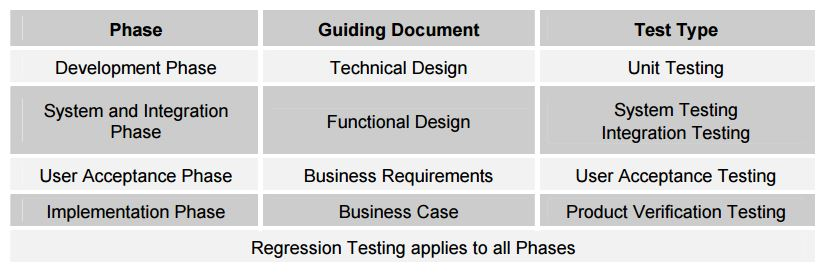
\includegraphics[scale=0.65]{SoftwareTesting.JPG}\\
        \caption{Types of software testing}
  \end{figure}
\begin{itemize}
\item \textbf{Black Box Testing}\\
Black box testing methods focus on the functional requirements in the software. That is, black box testing enables us to derive sets of input conditions that will fully exercise.\\
All functional requirements of the program Black box testing attempts to find errors in the following categories:
\begin{itemize}
\item Incorrect or missing function
\item	Interface errors
\item	Errors in data structure or external job access
\item	Performance errors
\item	Initialization and termination errors.
 
\end{itemize}
In the proposed application with the help of this technique, we do not use the code to determine a test suite; rather, knowing the problem that we are trying to solve, we come up with four types of test data: 
\begin{enumerate}
\item	Easy-to-compute data,
\item	Typical data,
\item	Boundary / extreme data,
\item	Bogus data.

\end{enumerate}

\item \textbf{Unit Testing}\\
Unit testing enables a programmer to detect error in coding. A unit test focuses verification of the smallest unit of software design. This testing was carried out during the coding itself. In this testing step, each module going to be work satisfactorily as the expected output from the module.\\

\noindent
The front end design consists of various forms. They were tested for data acceptance. Similarly, the back-end also tested for successful acceptance and retrieval of data. The unit testing is done on the developed code. Mainly the unit testing is done on modules.

\item \textbf{System Testing}\\
After performing the integration testing, the next step is output testing of the proposed system. No system could be useful if it doesn't produce the required output in a specified format. The outputs generated are displayed by the user. Here the output format is considered in to two ways. One in on screen and other in printed format.

\item \textbf{Integration Testing}\\
Through each program work individually, they should work after linking together. This is referred to as interfacing. Data may be lost across the interface; one module can have adverse effect on the other subroutines after linking may not do the desired function expected by the main routine. Integration testing is the systematic technique for constructing the program structure while at the same time conducting test to uncover errors associated with the interface. Using integrated test plan prepared in the design phase of the system development as a guide, the integration test was carried out. All the errors found in the system were corrected for the next testing step.

\item \textbf{User Acceptance Testing}\\
User Acceptance Testing is also called Beta testing, application testing, and end-user testing. Whatever you choose
to call it, it’s where testing moves from the hands of the IT department into those of the business users. Software
vendors often make extensive use of Beta testing, some more formally than others, because they can get users to do
it for free. \\

\noindent
By the time UAT is ready to start, the IT staff has resolved in one way or another all the defects they identified.
Regardless of their best efforts, though, they probably don’t find all the flaws in the application. A general rule of
thumb is that no matter how bulletproof an application seems when it goes into UAT, a user somewhere can still find a
sequence of commands that will produce an error. \\
\item \textbf{Product verification Testing}\\
Production verification testing is a final opportunity to determine if the software is ready for release. Its purpose is to
simulate the production cut-over as closely as possible and for a period of time simulate real business activity. As a
sort of full dress rehearsal, it should identify anomalies or unexpected changes to existing processes introduced by
the new application. For mission critical applications the importance of this testing cannot be overstated.\\

\noindent
The application should be completely removed from the test environment and then completely reinstalled exactly as it
will be in the production implementation. Then mock production runs will verify that the existing business process
flows, interfaces, and batch processes continue to run correctly. Unlike parallel testing in which the old and new
systems are run side-by-side, mock processing may not provide accurate data handling results due to limitations of
the testing database or the source data. 

\begin{table}[ht]
    \caption{Black-Box Test Plan of the Platform}
    \begin{tabular}{ |p{4cm}|p{4cm}|p{3cm}|p{4cm}|  }
    \hline
    \textbf{Component} & \textbf{Description} & \textbf{Input} & \textbf{Expected Output}\\
    \hline
    Proper Recognition of Command & To check command in English is recognised by Device as correctly & Vocal Command & Command is recognised by the device \\\hline

    Android Connectivity to Cloud DB & To check that data is transfered properly in both the direction to the Firebase Cloud DB with real-time results & Android App and Firebase Cloud DB & Android Application Updates are recognised by the platform\\\hline
    
    Performance of IOT Box & To check whether IOT Box performs correctly on the input of concerned commands & IOT Box Related Vocal Commands & IOT Box Works Seamlessly\\\hline
    
    Performance of Firebase Cloud & To check whether Firebase work with no downtime, real-time services and Provide API form Device and Android application  & Firebase Cloud DB & Firebase Cloud Db works as expected with Python and Android API\\\hline
    
    Response Of AI Device & To check whether the AI Device Vocal response to commands are correct & Vocal Commands along with required parameters & Output vocal command is the correct response to the input command\\\hline
    
    Integration test of the Platform & To check whether all the modules of the platform is working properly when interfaced together as one & All the modules if the platform & Data flows throughout the platform from one end to another without any errors\\
 
    \hline
    \end{tabular}
\end{table}
\end{itemize}





%\begin{table}[ht]
%\caption{Test Cases}
%\begin{tabular}{ |M{4cm}|p{5cm}|M{2.5cm}|M{3.2cm}|  }
% \hline
 %\textbf{USE CASE} & \textbf{FUNCTION BEING TESTED} & \textbf{INPUT} & \textbf{EXPECTED OUTPUT}\\
 %\hline
 
%Data Collection & Is data collected properly? & Web data & Stored records in DB\\

%\hline
 %Data Classification & Is data classified into  classes as per attributes? & Data in DB & Classes of attributes\\
 
 %\hline
 %Pattern identification & Is unique patterns generated? & Classes from classifier & Patterns as rules.\\
 
 %\hline
 %Prediction & Is regions having a common pattern? & Rules from apriori & Expected output\\
  
  %\hline
  
 
 %\end{tabular}
 
%\end{table}
%\end{comment}
